% Editable native annotations around unchanged verified IDE photographs.
\par
\begin{figure}[htbp]
  \centering
  \newsavebox{\MARScborpipelineregistersBox}
  \sbox{\MARScborpipelineregistersBox}{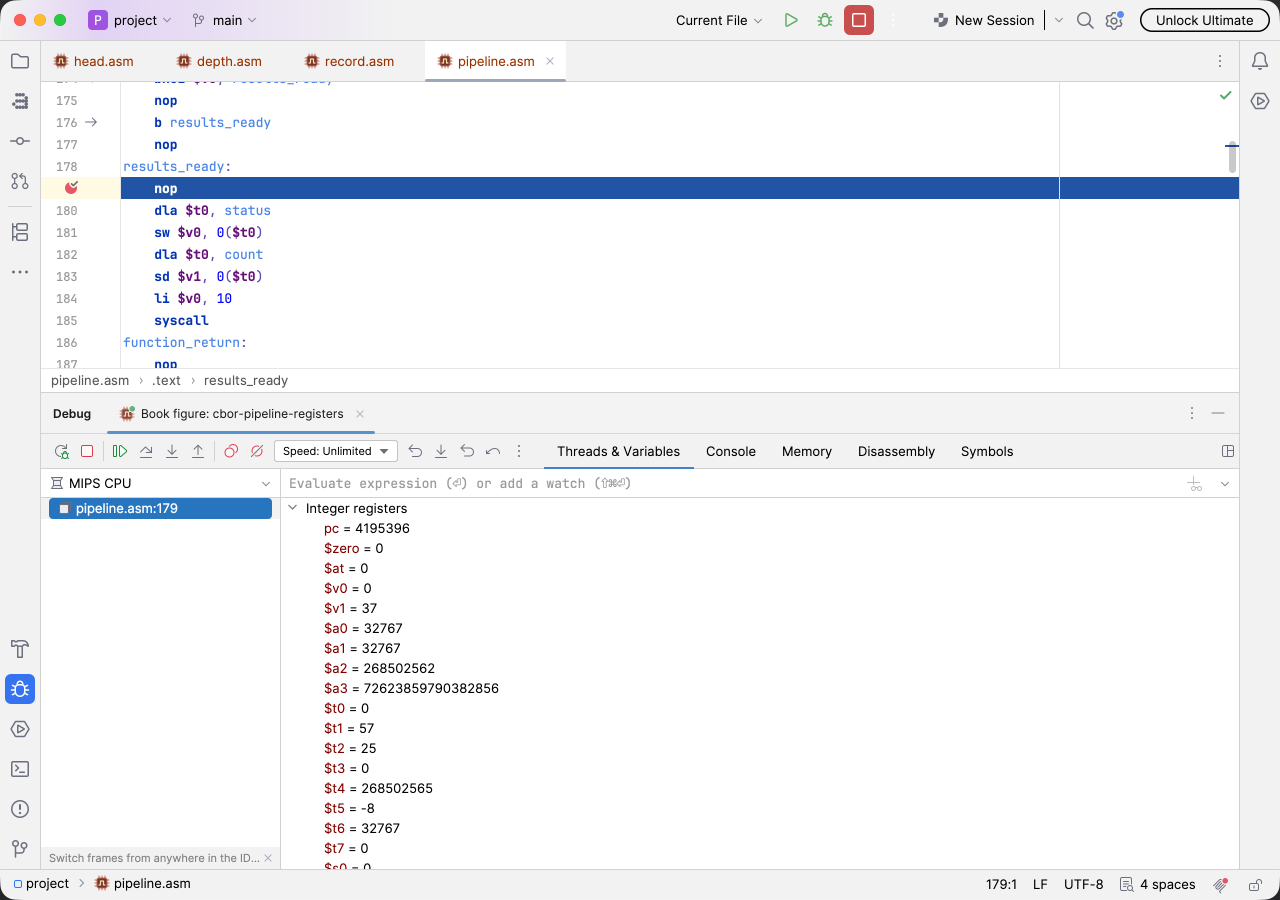
\includegraphics[artifact]{book/captures/032-cbor-telemetry/required-projection/registers.png}}
  \newsavebox{\MARScborpipelinesourceBox}
  \sbox{\MARScborpipelinesourceBox}{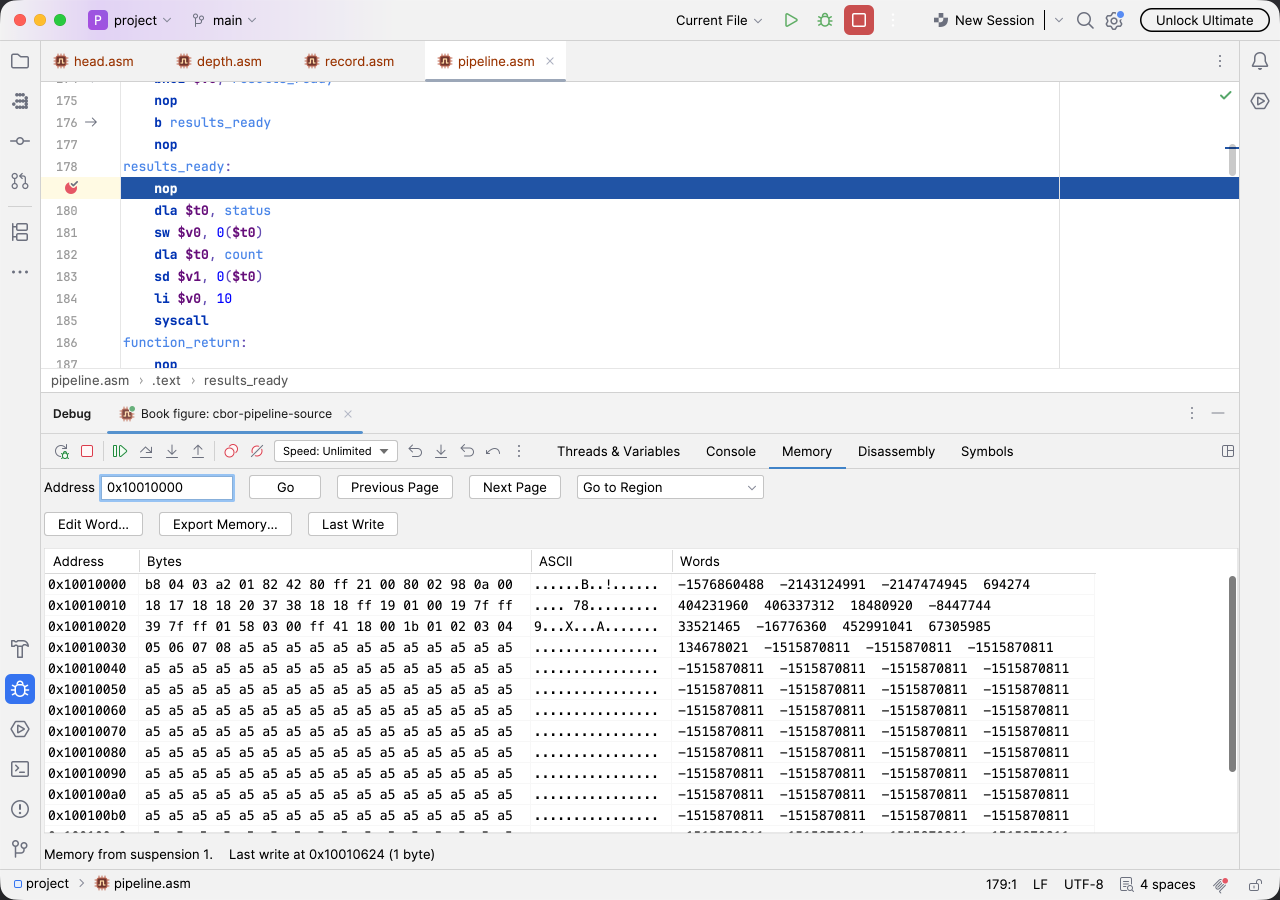
\includegraphics[artifact]{book/captures/032-cbor-telemetry/required-projection/source.png}}
  \newsavebox{\MARScborpipelineoutputBox}
  \sbox{\MARScborpipelineoutputBox}{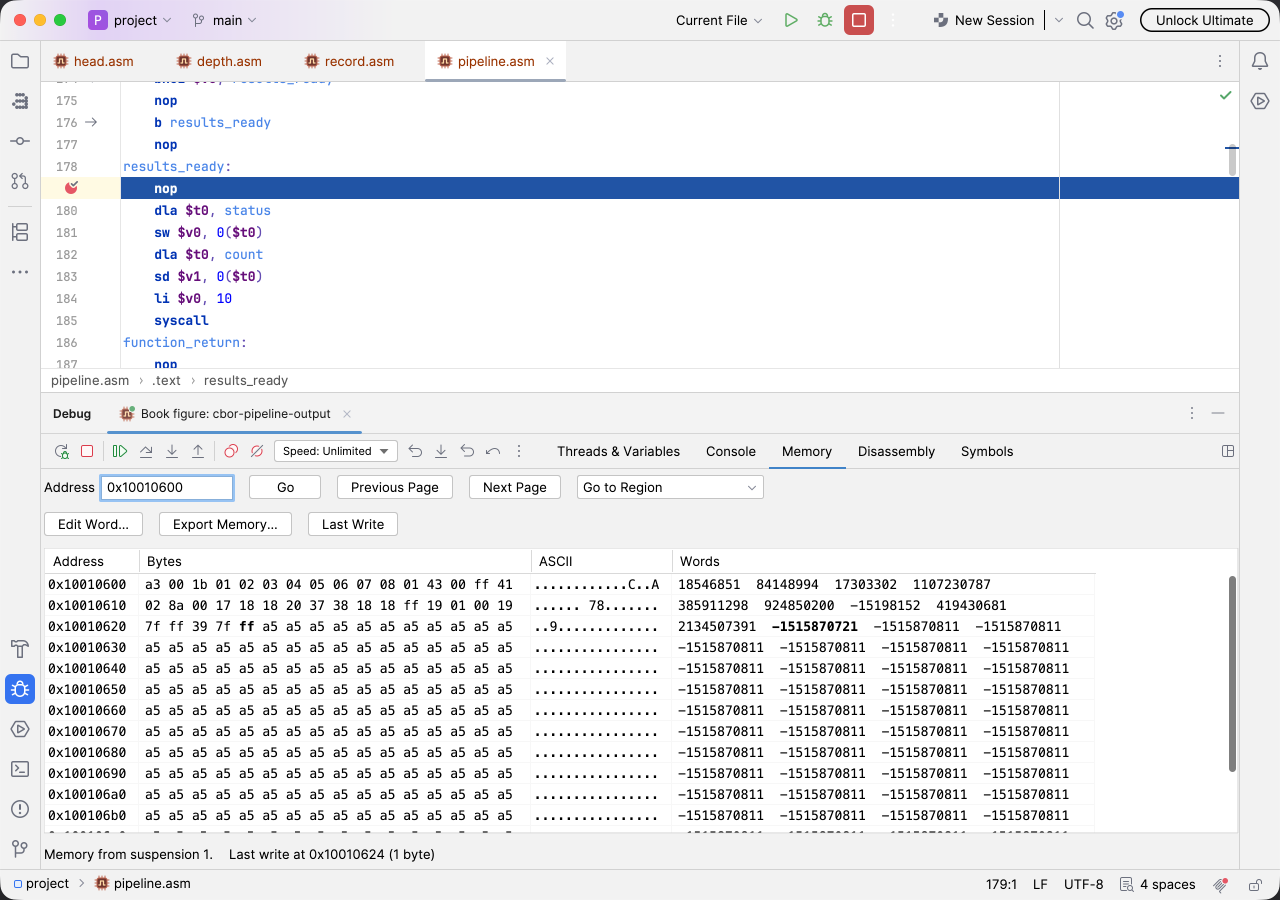
\includegraphics[artifact]{book/captures/032-cbor-telemetry/required-projection/output.png}}
  \edef\MARScborpipelinesourceLeft{\the\dimexpr0.036718750\wd\MARScborpipelineregistersBox\relax}
  \edef\MARScborpipelinesourceBottom{\the\dimexpr0.774444444\ht\MARScborpipelineregistersBox\relax}
  \edef\MARScborpipelinesourceRight{\the\dimexpr0.713281250\wd\MARScborpipelineregistersBox\relax}
  \edef\MARScborpipelinesourceTop{\the\dimexpr0.170000000\ht\MARScborpipelineregistersBox\relax}
  \edef\MARScborpipelinereturnsLeft{\the\dimexpr0.246093750\wd\MARScborpipelineregistersBox\relax}
  \edef\MARScborpipelinereturnsBottom{\the\dimexpr0.312222222\ht\MARScborpipelineregistersBox\relax}
  \edef\MARScborpipelinereturnsRight{\the\dimexpr0.553906250\wd\MARScborpipelineregistersBox\relax}
  \edef\MARScborpipelinereturnsTop{\the\dimexpr0.640000000\ht\MARScborpipelineregistersBox\relax}
  \edef\MARScborpipelineinputLeft{\the\dimexpr0.034375000\wd\MARScborpipelinesourceBox\relax}
  \edef\MARScborpipelineinputBottom{\the\dimexpr0.264444444\ht\MARScborpipelinesourceBox\relax}
  \edef\MARScborpipelineinputRight{\the\dimexpr0.584375000\wd\MARScborpipelinesourceBox\relax}
  \edef\MARScborpipelineinputTop{\the\dimexpr0.608888889\ht\MARScborpipelinesourceBox\relax}
  \edef\MARScborpipelineoutputLeft{\the\dimexpr0.034375000\wd\MARScborpipelineoutputBox\relax}
  \edef\MARScborpipelineoutputBottom{\the\dimexpr0.287777778\ht\MARScborpipelineoutputBox\relax}
  \edef\MARScborpipelineoutputRight{\the\dimexpr0.584375000\wd\MARScborpipelineoutputBox\relax}
  \edef\MARScborpipelineoutputTop{\the\dimexpr0.608888889\ht\MARScborpipelineoutputBox\relax}
  \begin{tikzpicture}[alt={Four details at results_ready show success and output length thirty-seven, the original fifty-two-byte four-pair map, and a three-pair deterministic encoding ending before its unchanged backing suffix.}]
    \node[anchor=north west,inner sep=0,font=\small\bfseries] (source-title) at (6mm,0) {Before the caller saves results};
    \node[anchor=north west,inner sep=0] (source) at ([yshift=-1mm]source-title.south west) {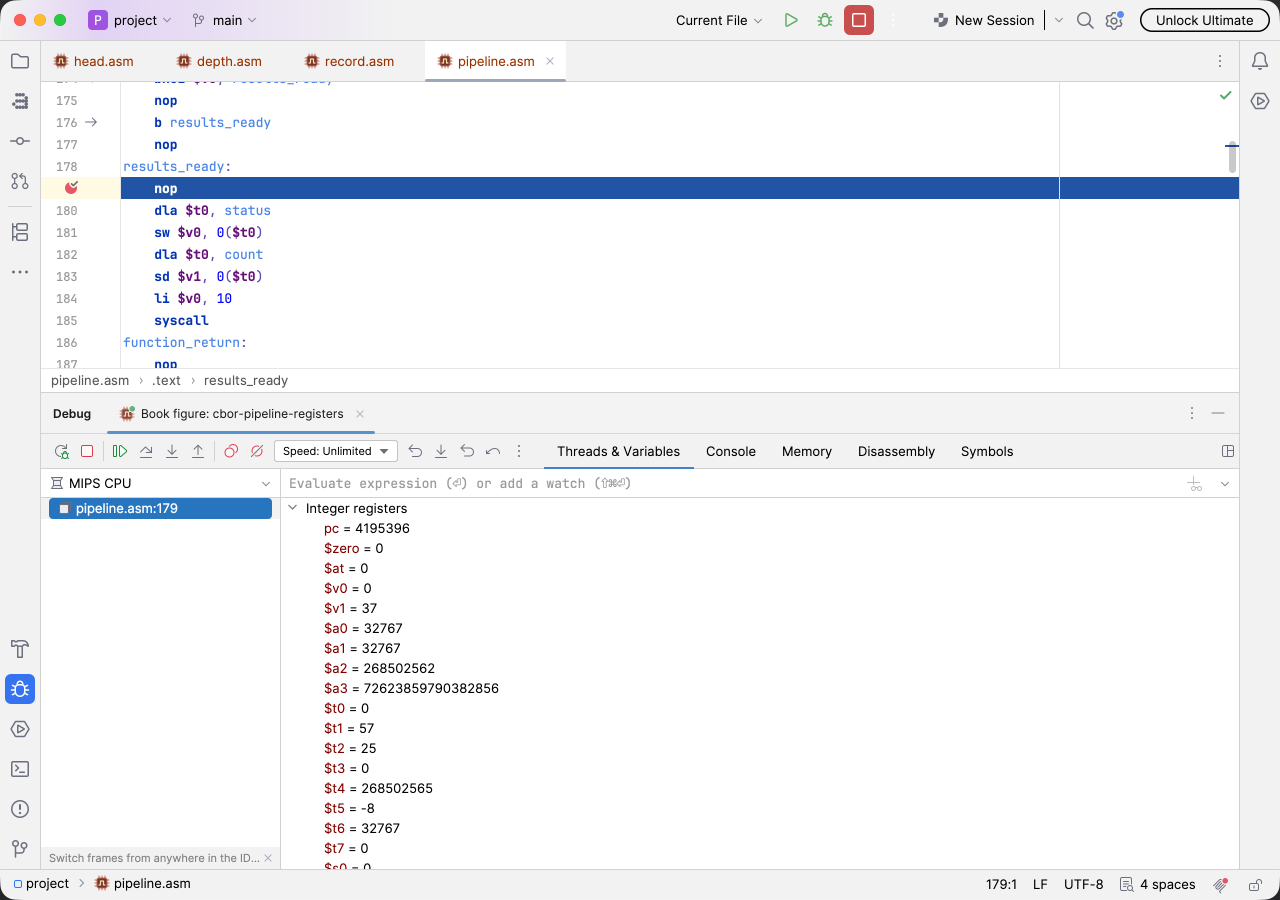
\includegraphics[width=0.54\linewidth,artifact,trim={\MARScborpipelinesourceLeft{} \MARScborpipelinesourceBottom{} \MARScborpipelinesourceRight{} \MARScborpipelinesourceTop{}},clip]{book/captures/032-cbor-telemetry/required-projection/registers.png}};
    \begin{scope}[shift={(source.south west)},x={($(source.south east)-(source.south west)$)},y={($(source.north west)-(source.south west)$)}]
      \draw[black,line width=0.7pt] (0.237500000,0.080000000) rectangle (0.406250000,0.520000000);
      \node[draw=black,fill=white,circle,inner sep=1.5pt,font=\footnotesize] at ($(0.237500000,0.520000000)+(-3mm,0)$) {1};
    \end{scope}
    \node[anchor=north west,inner sep=0,font=\small\bfseries] (returns-title) at ([yshift=-1mm]source.south west) {Success and encoded output length};
    \node[anchor=north west,inner sep=0] (returns) at ([yshift=-1mm]returns-title.south west) {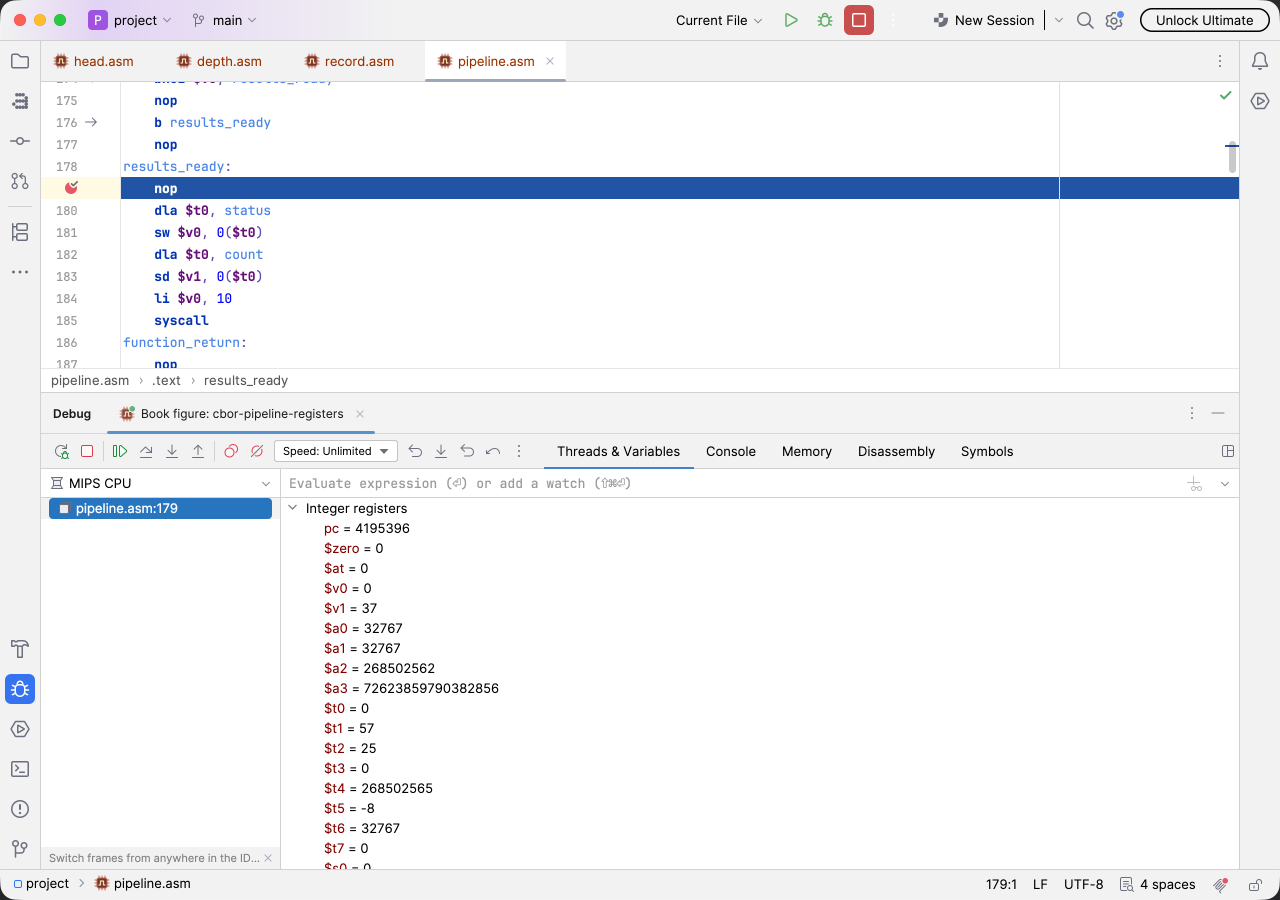
\includegraphics[width=0.48\linewidth,artifact,trim={\MARScborpipelinereturnsLeft{} \MARScborpipelinereturnsBottom{} \MARScborpipelinereturnsRight{} \MARScborpipelinereturnsTop{}},clip]{book/captures/032-cbor-telemetry/required-projection/registers.png}};
    \begin{scope}[shift={(returns.south west)},x={($(returns.south east)-(returns.south west)$)},y={($(returns.north west)-(returns.south west)$)}]
      \draw[black,line width=0.7pt] (0.023437500,0.023255814) rectangle (0.250000000,0.953488372);
      \node[draw=black,fill=white,circle,inner sep=1.5pt,font=\footnotesize] at ($(0.023437500,0.953488372)+(-3mm,0)$) {2};
    \end{scope}
    \node[anchor=north west,inner sep=0,font=\small\bfseries] (input-title) at ([yshift=-1mm]returns.south west) {Complete input and backing suffix};
    \node[anchor=north west,inner sep=0] (input) at ([yshift=-1mm]input-title.south west) {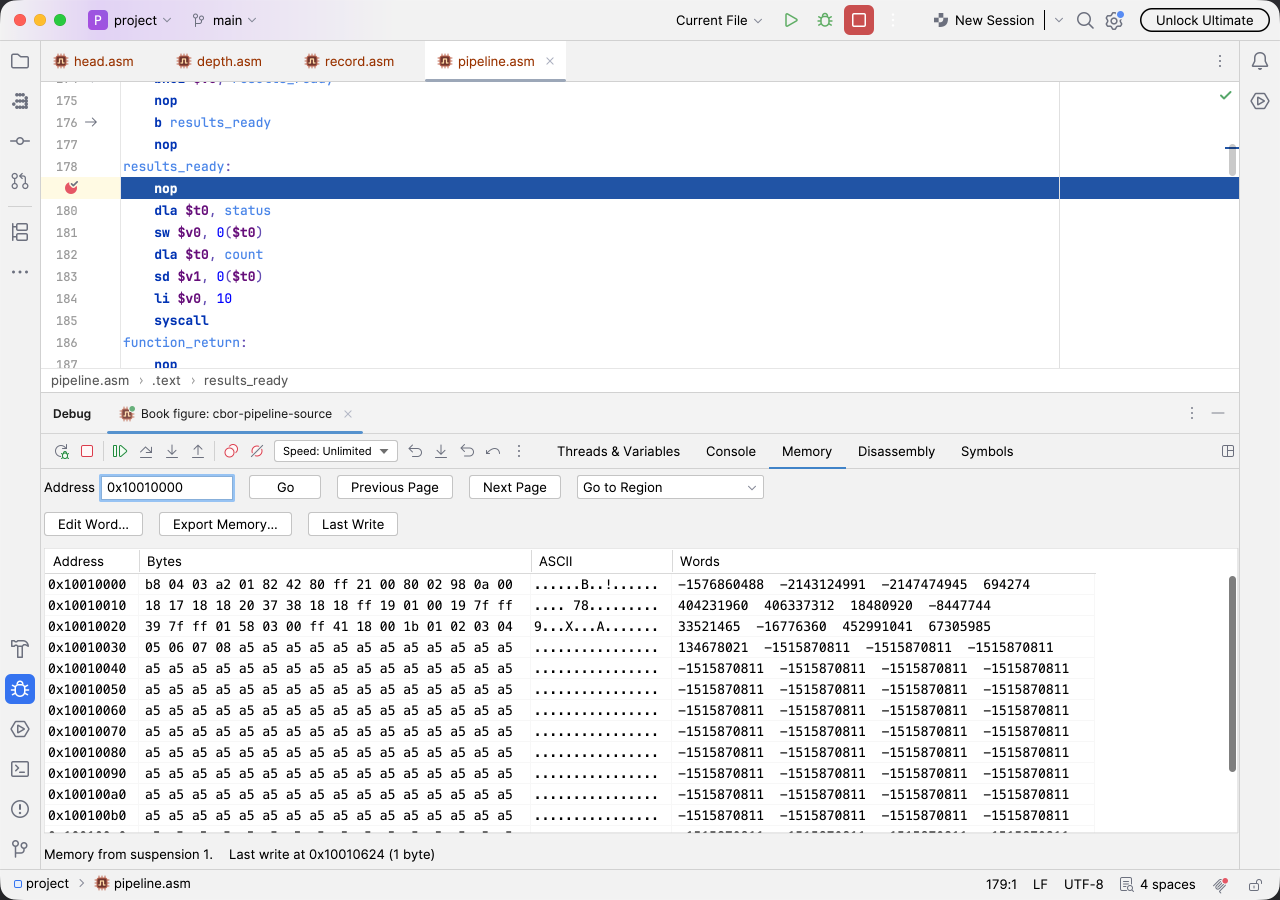
\includegraphics[width=0.84\linewidth,artifact,trim={\MARScborpipelineinputLeft{} \MARScborpipelineinputBottom{} \MARScborpipelineinputRight{} \MARScborpipelineinputTop{}},clip]{book/captures/032-cbor-telemetry/required-projection/source.png}};
    \begin{scope}[shift={(input.south west)},x={($(input.south east)-(input.south west)$)},y={($(input.north west)-(input.south west)$)}]
      \draw[black,line width=0.7pt] (0.194672131,0.035087719) rectangle (0.997950820,0.771929825);
      \node[draw=black,fill=white,circle,inner sep=1.5pt,font=\footnotesize] at ($(0,0.771929825)+(-3mm,0)$) {3};
    \end{scope}
    \node[anchor=north west,inner sep=0,font=\small\bfseries] (output-title) at ([yshift=-1mm]input.south west) {Required-field encoding and untouched suffix};
    \node[anchor=north west,inner sep=0] (output) at ([yshift=-1mm]output-title.south west) {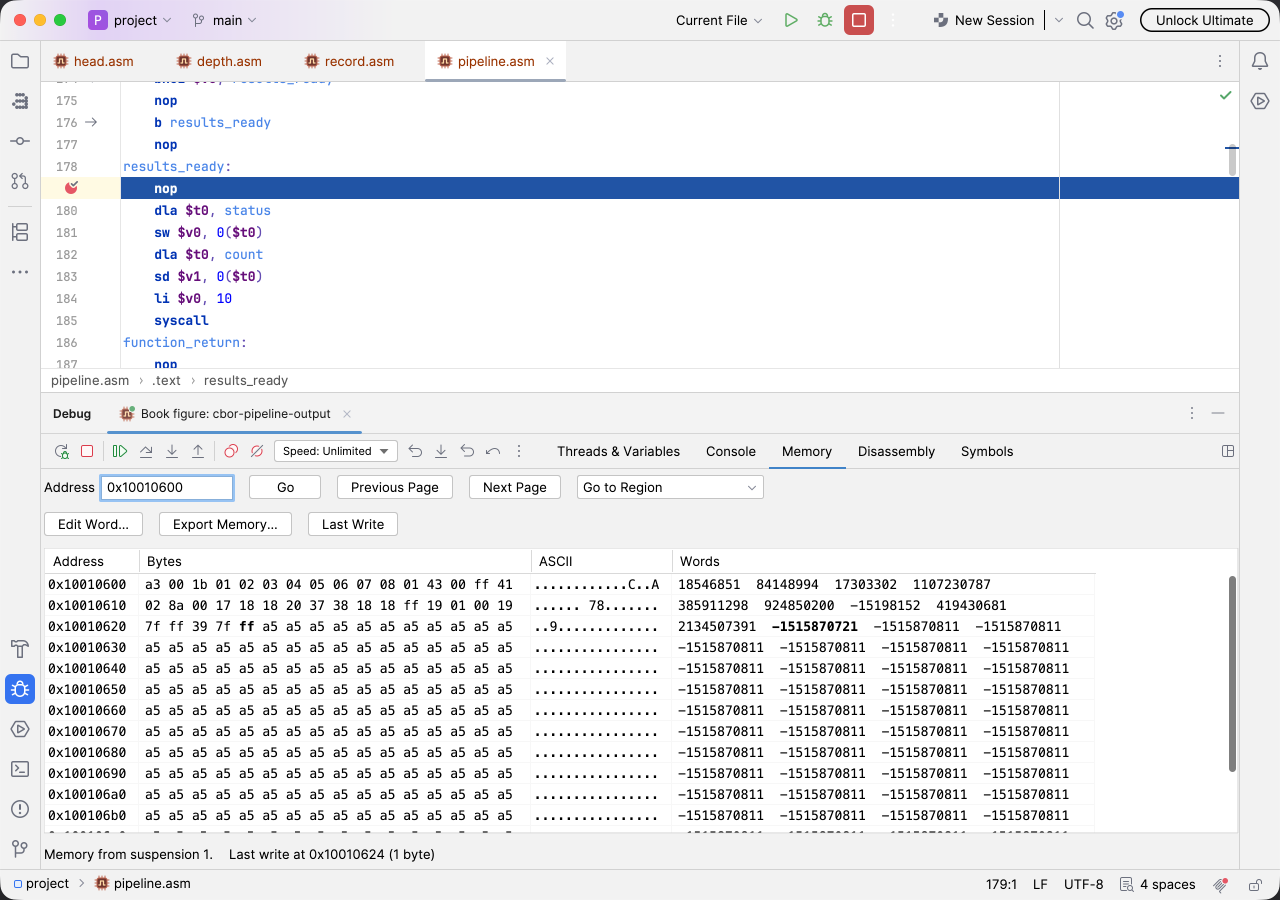
\includegraphics[width=0.84\linewidth,artifact,trim={\MARScborpipelineoutputLeft{} \MARScborpipelineoutputBottom{} \MARScborpipelineoutputRight{} \MARScborpipelineoutputTop{}},clip]{book/captures/032-cbor-telemetry/required-projection/output.png}};
    \begin{scope}[shift={(output.south west)},x={($(output.south east)-(output.south west)$)},y={($(output.north west)-(output.south west)$)}]
      \draw[black,line width=0.7pt] (0.194672131,0.043010753) rectangle (0.997950820,0.720430108);
      \node[draw=black,fill=white,circle,inner sep=1.5pt,font=\footnotesize] at ($(0,0.720430108)+(-3mm,0)$) {4};
    \end{scope}
  \end{tikzpicture}
  \par\smallskip
  \begin{minipage}{\linewidth}
    \small
    \begin{enumerate}
      \setlength{\itemsep}{0pt}
            \setlength{\parsep}{0pt}
      \item At \texttt{results\_ready}, head reading, complete walking, decoding, sizing and encoding have returned. The selected \texttt{nop} precedes the caller stores that retain status and count.
      \item \texttt{v0 = 0} reports success. \texttt{v1 = 37} counts encoded output bytes. The earlier head result was two bytes and the decoder result fifty-two; each count measures its declared extent.
      \item The input begins \texttt{b8 04}: four map pairs in an accepted nonpreferred head form. Optional key three and its nested value must validate even though the output omits them. The final twelve \texttt{a5} bytes shown are backing storage after the fifty-two-byte input.
      \item The output begins \texttt{a3}, the shortest head for three map pairs. Keys zero, one and two retain the complete counter, binary identifier and readings. The last five logical output bytes occupy the final displayed row; subsequent \texttt{a5} bytes are untouched. Independent decoding and canonical encoding confirm the same required-field values. This is a schema projection, not a byte-for-byte copy of the input.
    \end{enumerate}
  \end{minipage}
  \caption{The pipeline validates optional metadata and emits the required fields in deterministic form.}
  \label{capture:032-cbor-telemetry-required-projection}
  \label{cbor-required-projection}
\end{figure}
\par
